\section{A Simple Example}


\begin{figure}
\begin{center}
{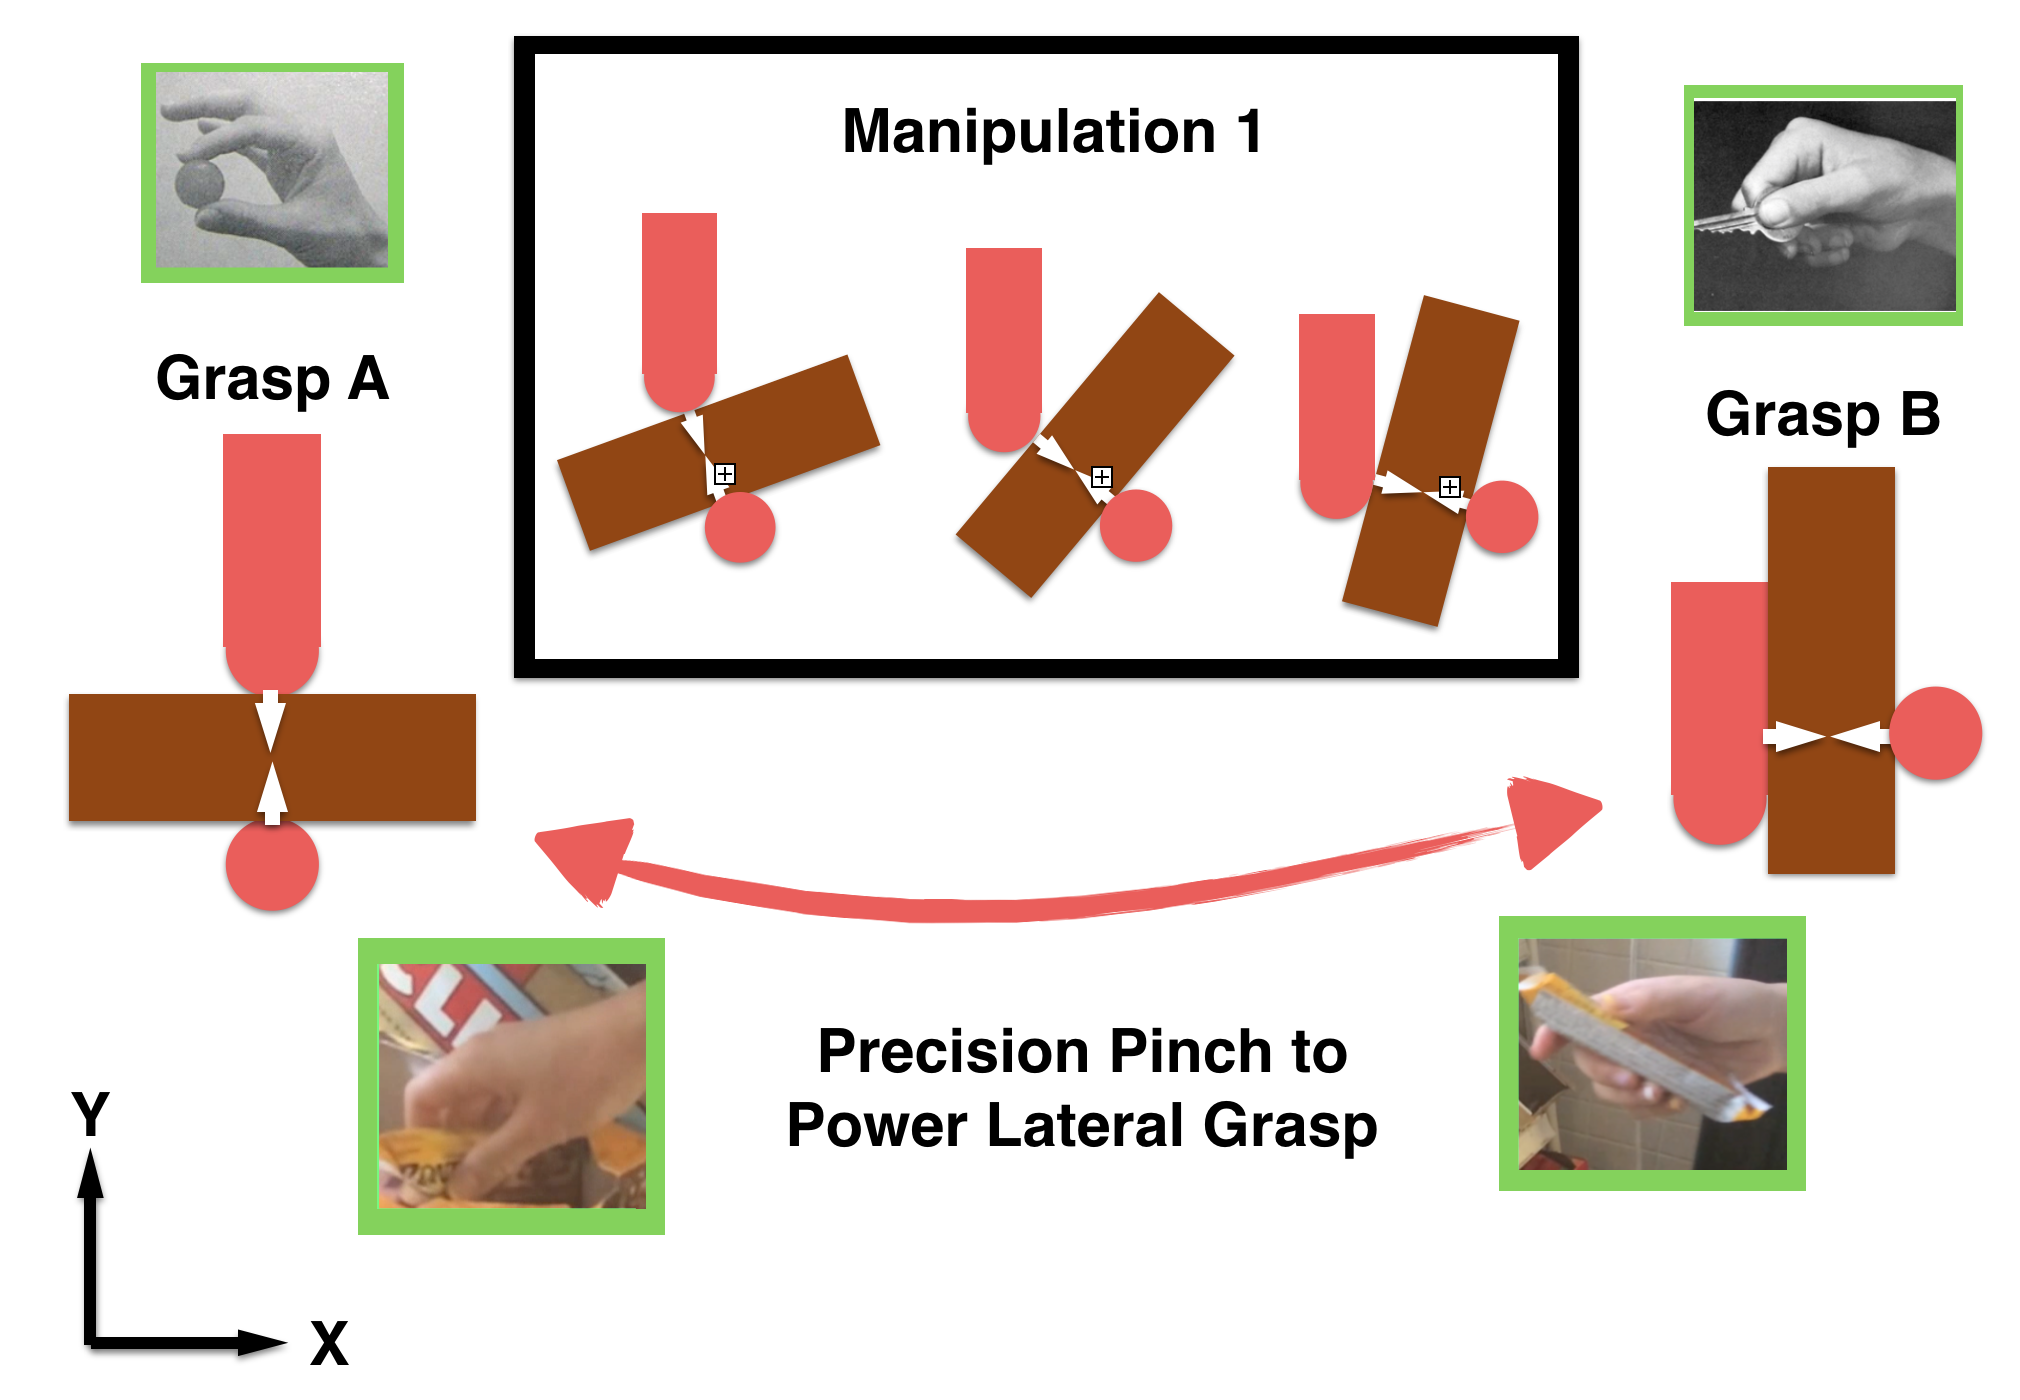
\includegraphics[width=4in]{./figs/simpleExample.png}}
\end{center}
\vspace*{-0.3in}
\caption[]{This trivial Grasp Net nonetheless captures two important grasps and a dexterous motion to move between them.}
\label{SimpleGraspNet}
\end{figure}

Consider the trivial Grasp Net shown in Figure~\ref{SimpleGraspNet}.     This figure shows two grasps.   Grasp A (Left) is a precision pinch grasp, typical for lifting objects from a surface, placing them down, performing certain dexterous actions such as using tweezers, and as a staging point for moving to other grasps.   We observe that many objects are initially acquired from a surface in a pinch grasp and then moved to a final grasp that is more useful, comfortable, or powerful.    Forces in the pinch grasp oppose one another along the local y-axis.   

Grasp B (Right) is a lateral grasp, often called the key pinch grasp, useful for comfortably and securely holding objects, for certain assembly operations (e.g., put a key or a card into a slot), and for offering an object to a person (or another robot).   Forces for the lateral grasp in this example oppose one another along the x-axis.  Greater forces may be desired for this grasp.   

Manipulation 1 is used to move between the two grasps.   In this case we can imagine the "thumb" pivoting around the "index finger," although in our final design, the motion may be generated by either or both fingers.    The variation in object widths creates a family of curves describing motion of the thumb relative to the finger.   The manipulation is specified to utilize sliding contact on the finger and rolling frictional contact with the thumb.  There is a collection of benchmark objects of varying width, required grasp force, and other physical properties.   The design problem is to choose degrees of freedom, place actuators and joint limits, and select passive compliance for the mechanism.  A successful design must be able to accomplish Grasp A, Grasp B, and Manipulation 1 easily / robustly / reliably in the presence of uncertainties.

Figure 2 shows one solution that was derived based on the goal of minimizing the total number of actuators and the number of actuators per finger while ensuring that the mechanism could accomplish the task.  This design relies on spring forces to close the fingers at both Grasp A and Grasp B, while using actuators to open the fingers.   If both actuators are engaged briefly in a coordinated way, the grasp can be shifted from A to B or from B to A, performing Manipulation 1 in both directions.   The coordination could be done mechanically for some range of objects, leading to a one actuator system.   Such a system would be reminiscent of a body-powered prosthesis with a voluntary-opening end effector \cite{smith2004atlas}.   However, instead of a single available grasp, we have been able to accomplish two different grasps and a dexterous manipulation between them.
A physical instantiation of this solution is shown in Figure \ref{SimpleExampleResults}.   It was 3D printed and assembled in a matter of hours.

\begin{figure}
\begin{center}
{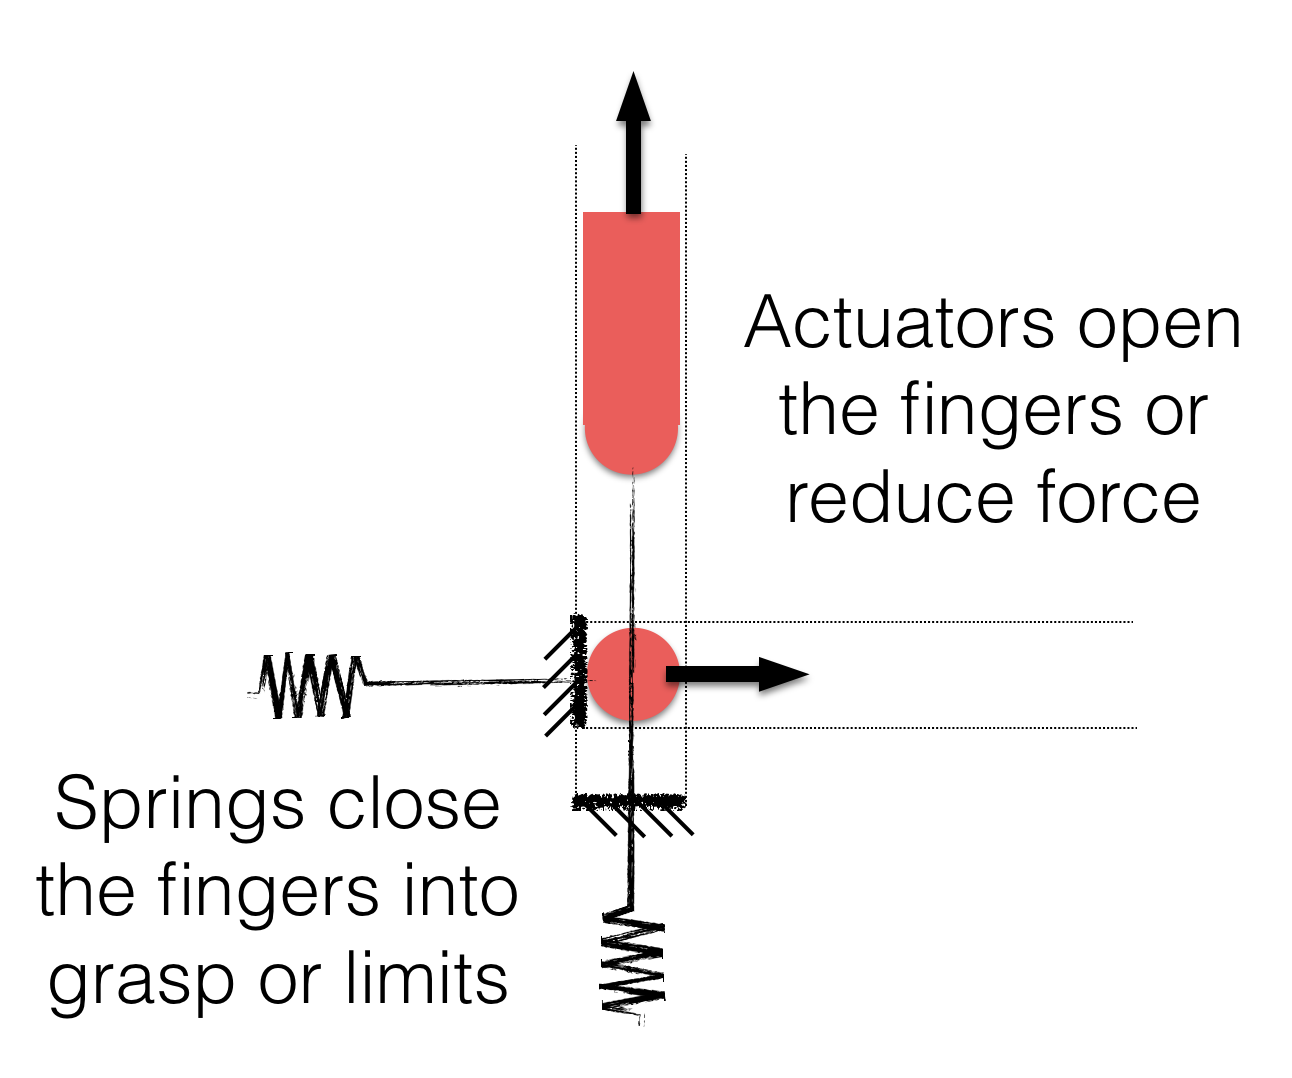
\includegraphics[width=3in]{./figs/springCloseDesign.png}}
{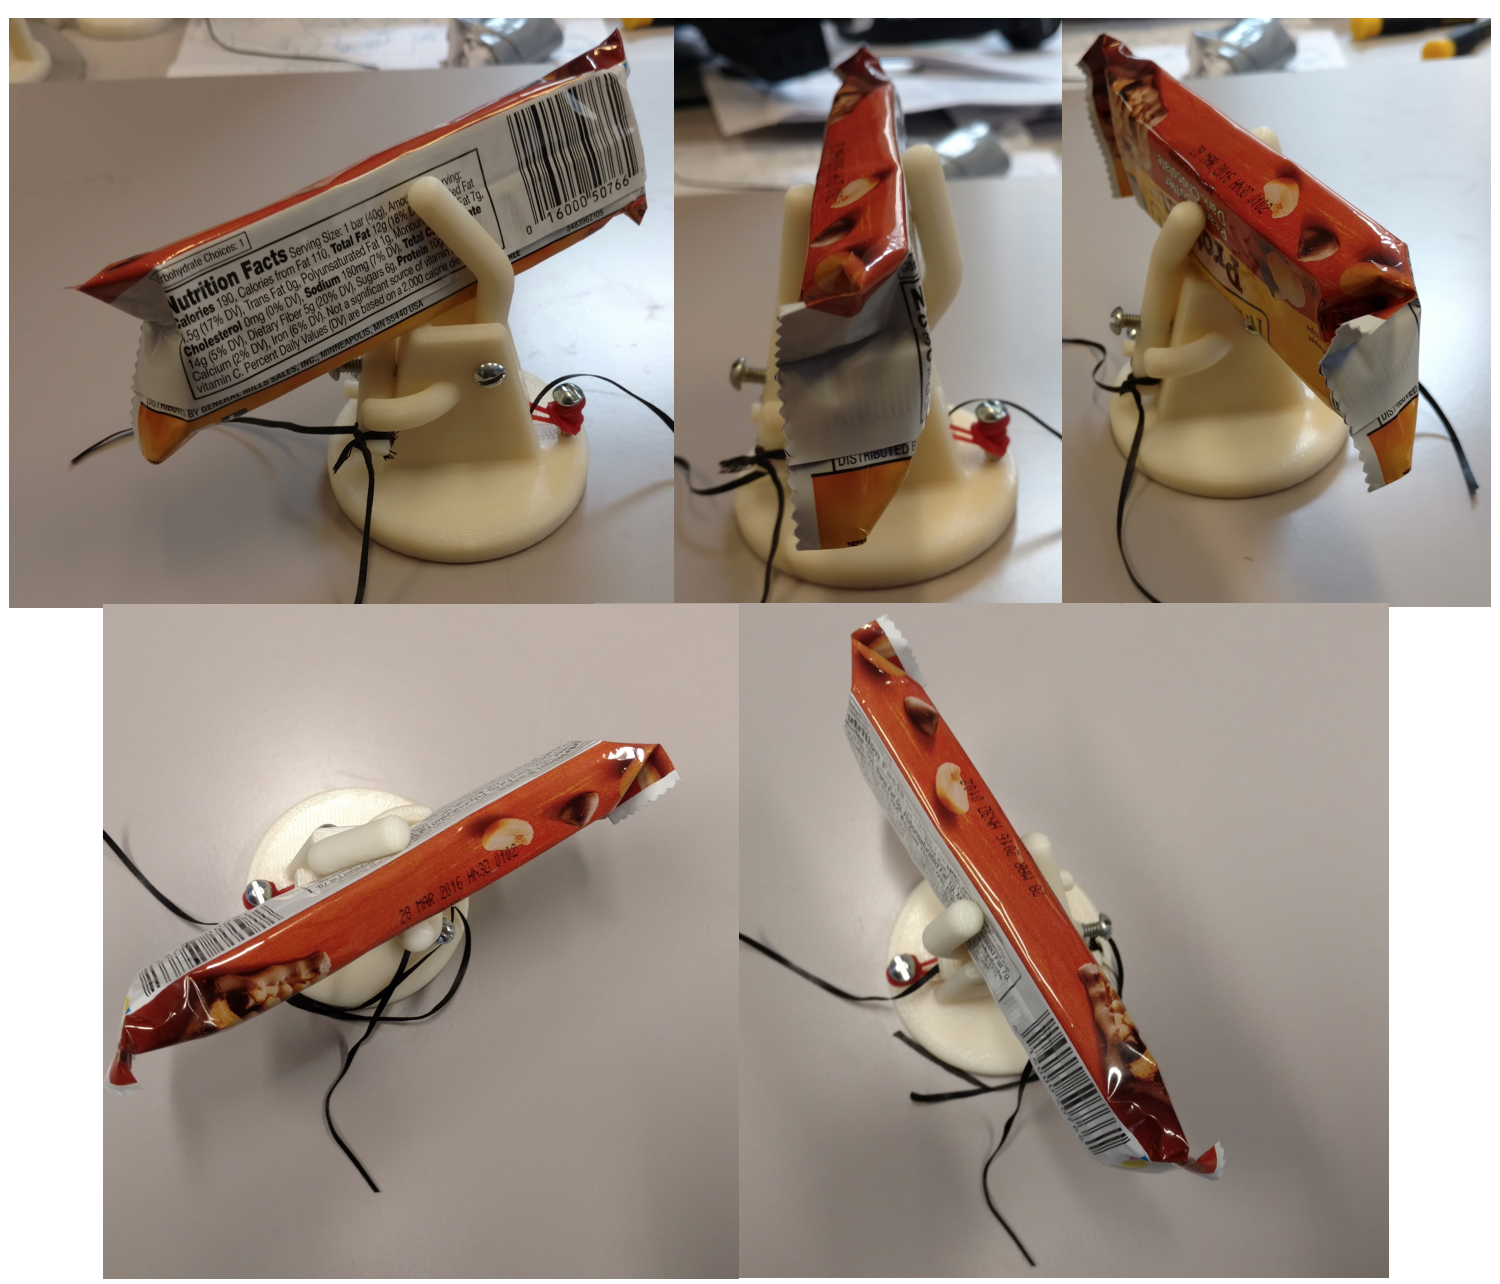
\includegraphics[width=3in]{./figs/testManipulator.png}}
\end{center}
\vspace*{-0.2in}
\caption[]{(Left) One final solution.  (Right) A physical implementation that approximates this design with 3D printed base and fingers.}
\label{SimpleExampleResults}
\end{figure}


